\documentclass{standalone}
\usepackage{pgfplots}
\usetikzlibrary{shapes.geometric, intersections}
\pgfplotsset{compat=1.7}

\begin{document}
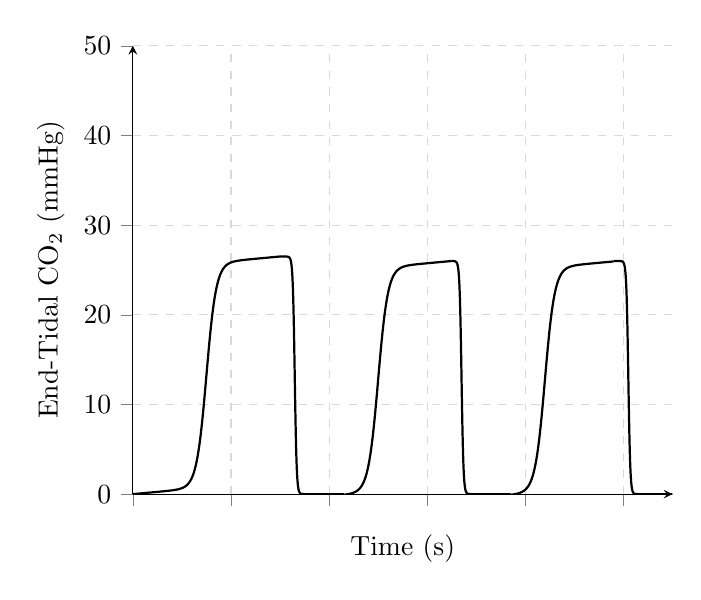
\begin{tikzpicture}

    \begin{axis}[
axis x line=bottom,
  axis y line=left,
	ymin = 0,
	ymax = 50,
	xmin = 0,
xmax = 110,
        grid = major,
        grid style={dashed, gray!30},
	 ylabel near ticks,
	xlabel near ticks,
	xticklabels={},
        xlabel=Time (s),
        ylabel=End-Tidal CO\textsubscript{2} (mmHg),
        tick align=outside,
        enlargelimits=false,]

 \addplot[domain=0:30, black, thick,samples=500] {25*(1/(1+exp(-1*(x-15))))+0.05*x};
 \addplot[domain=30:43, black, thick,samples=500] {26.5*(1/(1+exp(5*(x-33))))};

 \addplot[domain=43:65, black, thick,samples=500] {25*(1/(1+exp(-1*(x-50))))+0.05*(x-45)};
 \addplot[domain=65:77, black, thick,samples=500] {26*(1/(1+exp(5*(x-67))))};

 \addplot[domain=43:98, black, thick,samples=500] {25*(1/(1+exp(-1*(x-84))))+0.05*(x-79)};
 \addplot[domain=98:110, black, thick,samples=500] {26*(1/(1+exp(5*(x-101))))};





\end{axis}

\end{tikzpicture} 
\end{document}